\documentclass[12pt,a4paper]{report}
\usepackage[utf8]{inputenc}
\usepackage[english]{babel}
\usepackage[T1]{fontenc}
\usepackage{amsmath}
\usepackage{amsfonts}
\usepackage{amssymb}
\usepackage{lmodern}
\usepackage{authoraftertitle}
\usepackage[final]{graphicx}
\DeclareGraphicsExtensions{.pdf,.png,.jpg}
\usepackage{color}
\usepackage{hyperref}
\hypersetup{
	colorlinks=true,
	linkcolor=black,
	urlcolor=red,
	citecolor=black,
	linktoc=all
}

%Header & Footer
%\usepackage{lastpage}
%\rfoot{\thepage\ of \pageref{LastPage}}



\date{29.09.2014}
\author{Ari Ayvazyan}
\title{JEE Security Structure Part 1}

\begin{document}

\maketitle
\tableofcontents


\chapter{\MyTitle}
%\begin{flushright}
%        \MyAuthor, \MyDate
%\end{flushright}


\section{Introduction to Security Architecture}
Most web applications have a few things in common:\\
They need to figure out who is the user that is using the application and what is he allowed to do and see.\\
According to Oracle, there are two ways to implement such functionality.\cite{oracleDoc}//
\begin{enumerate}
	\item Programmatic
	\item Declarative (this includes Annotations and XML-Files)
\end{enumerate}


\begin{figure}[h]
\centering
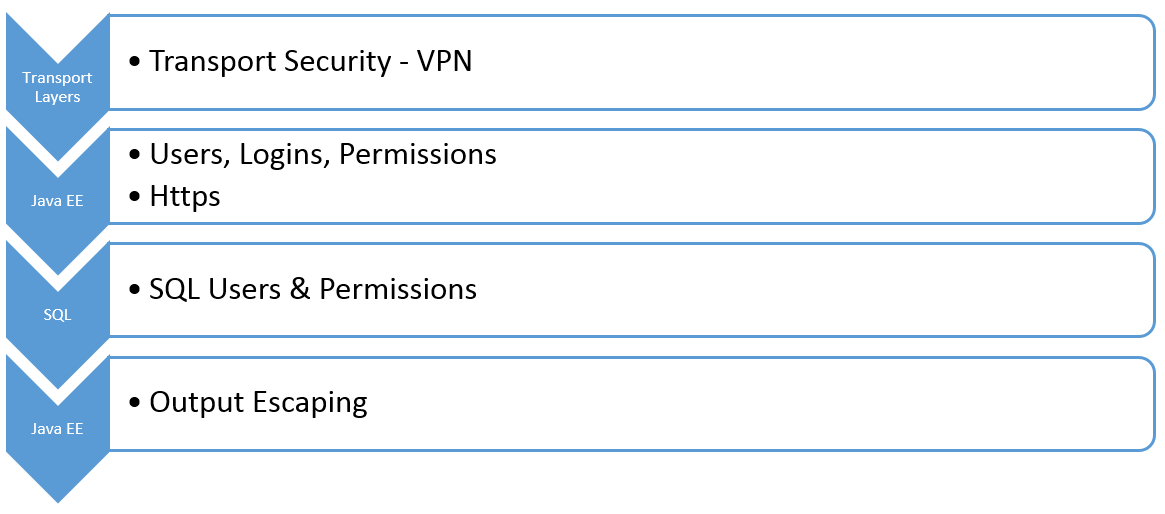
\includegraphics[width=1\linewidth]{res/SecurityLayers}
\caption{Security Layers in a common JEE application}
\label{fig:SecurityLayers}
\end{figure}


\section{Authentication}
Authentication\\
Who are you?\\
Identification\\

\section{Authorization}
Authorization\\
What are you allowed to do?\\
Assignment of Permissions to a Authenticated User\\


\section{Deployment Descriptors}
Describes how the Application should be Deployed.\\
Defines Security Constraints\\
\begin{itemize}
	\item Protected Information
	\item Probably SSL
	\item Specify which user may access them
\end{itemize}
Deployment Descriptors are XML-Files\\
Usually located in /WEB-INF/\\
\begin{itemize}
	\item web.xml
	\item Vendor-specific.xml (E.g. Glassfish: glassfish-web.xml)
\end{itemize}

\subsection*{web.xml}
Protected Resources\\
Security Roles\\
Authentication methods\\

\subsection*{(vendor-specific).xml}
User – Role mapping\\
Group – Role mapping\\
\\
Vendor specific settings\\

\section{Principals}
A Principal is a identity that can be authenticated.\\
E.g. a Unique user name\\

\section{Credential}
A Credential is defined as information that is used to authenticate a Principal.\\
E.g. a Password\\

\section{Groups}
Groups and Principals can be mapped to Roles.\\
Groups are defined in vendor-specific.xml\\

\section{Roles}
Permissions are granted to Roles.\\
Roles are defined in the web.xml file\\

\section{Realms}
aka Security policy domain\\
Provides information about principals, their Groups and their credentials\\
May be a Database, File structure, connection…\\\\
In other words:\\
It contains user information\\
E.g. Username, Password \& Permissions\\

\newpage
\section{Implementation sample}
\href{https://github.com/aayvazyan-tgm/JavaEESecurityExample}{https://github.com/aayvazyan-tgm/JavaEESecurityExample}\\
\begin{figure}[h!]
\centering
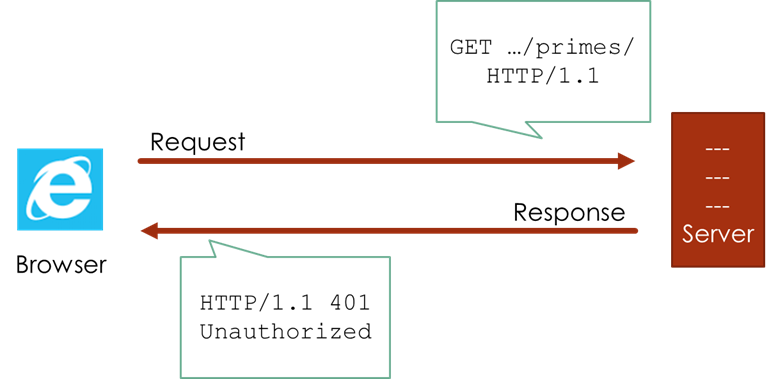
\includegraphics[width=1\linewidth]{res/Unauthorized}
\caption{The user tries to access a resource without authentication}
\label{fig:Unauthorized}
\end{figure}

\begin{figure}[h!]
	\centering
	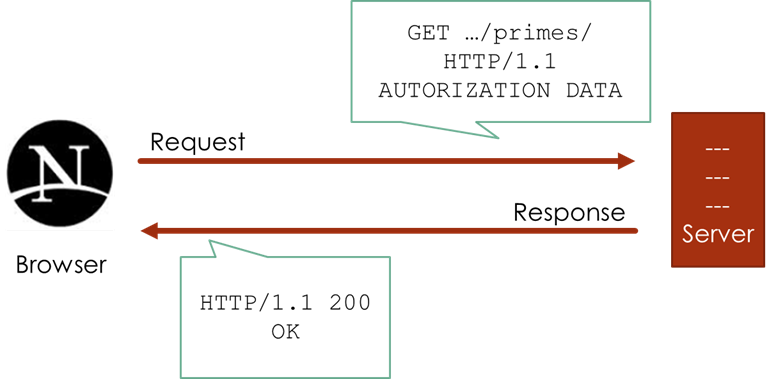
\includegraphics[width=1\linewidth]{res/Authorized}
	\caption{The user sends authentication data with his request}
	\label{fig:Authorized}
\end{figure}

\section{Frameworks}
\subsection{Shiro}
Offers: Authentication, Authorization, Cryptography\\
Simple to use\\\\
Advantages/Disadvantages\\
Implementation Sample

\subsection{Spring}
Offers: Authentication, Authorization, Cryptography\\
Very structured\\\\
Advantages/Disadvantages\\

\subsection{JAAS - Java Authentication and Authorization Service}
Offers: Authentication, Authorization, Cryptography\\
Included in Java SE since Java 1.4 (javax.security.auth)\\\\
Advantages/Disadvantages\\

\section{Output escaping}
Escape user input to prevent injections.\\
\\
Escape the output to add a extra layer of security.\\
Use a Framework to do so!\\

\section{Whats to come in Part 2 (Adrian)}
\begin{itemize}
	\item Working with Digital Certificates\\
	\item Securing Application Clients\\
	\item Security with Enterprise Beans\\
	\item Further Framework Information\\
\end{itemize}


\newpage
\begin{thebibliography}{99}
\bibitem{JavaOne}JavaOne 2014: The Anatomy of a Secure Web Application Using Java, \\
Shawn McKinney \& John Field, September 29, 2014\\
San Francisco
\bibitem{jSecVvulnerabilities}Java Security: Sicherheitslücken identifizieren und vermeiden, \\
Marc Schönefeld, 1. edition 2011\\
Publisher: Hüthig Jehle Rehm GmbH, Heidelberg. \\
ISBN/ISSN 978-3-8266-9105-8
\bibitem{EJSec}Enterprise Java Security: Building Secure J2EE Applications,\\
Marco Pistoia, Nataraj Nagaratnam, Larry Koved, Anthony Nadalin,\\
1. edition 2004 \\
Publisher: Addison-Wesley Professional.\\
ISBN/ISSN: ISBN 0-321-11889-8
\bibitem{oracleDoc}Official JavaEE Documentation, Oracle,\\
29.09.2014
http://docs.oracle.com/javaee/7/tutorial/partsecurity.htm\#GIJRP
Java EE 6,\\
Dirk Weil, 1. edition 2012\\
Publisher: entwickler.press\\
ISBN 978-3-86802-077-9
\bibitem{jeecookbook}Java EE 6 Cookbook for Securing, Tuning, and Extending Enterprise Applications,\\
Mick Knutson,\\
1. edition June 2012 \\
Publisher: Addison-Wesley Professional.\\
ISBN/ISSN: ISBN 9781849683166
\end{thebibliography}
\end{document}
